\documentclass[border=4pt]{standalone}
\usepackage{tikz}
\usepackage{pgfplots}
\pgfplotsset{compat=1.18}
\usetikzlibrary{shapes.geometric,arrows.meta,positioning,calc,fit,decorations.pathreplacing,backgrounds}
\definecolor{boxblue}{RGB}{225,238,252}
\definecolor{boxgreen}{RGB}{225,247,231}
\definecolor{boxorange}{RGB}{253,236,216}
\definecolor{boxgray}{RGB}{237,237,237}
\definecolor{boxred}{RGB}{253,226,226}
\begin{document}
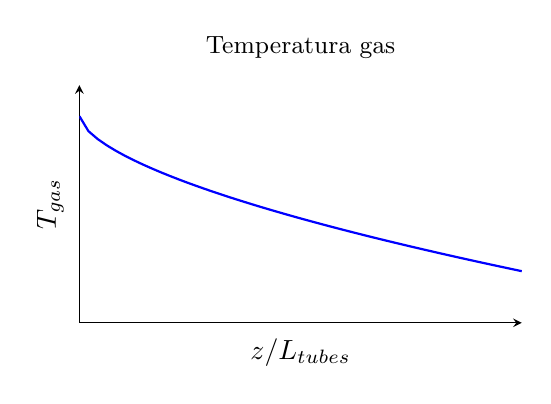
\begin{tikzpicture}
\begin{axis}[
  width=7.2cm, height=4.6cm,
  xlabel={$z/L_{tubes}$}, ylabel={$T_{gas}$},
  xtick=\empty, ytick=\empty,
  axis lines=left,
  ymin=0, ymax=1.15, xmin=0, xmax=1,
  title={\small Temperatura gas},
]
\addplot[thick,blue,domain=0:1,samples=50]{1 - 0.75*x^0.6};
\end{axis}
\end{tikzpicture}
\hspace{0.4cm}
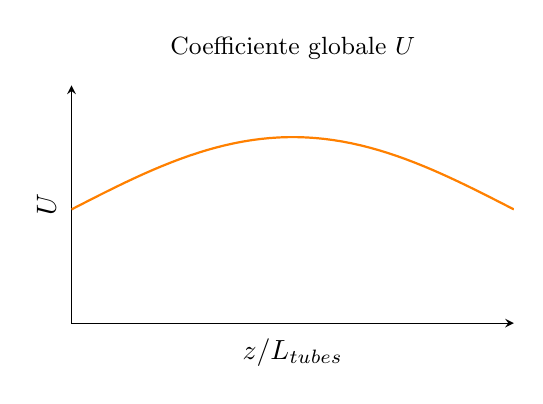
\begin{tikzpicture}
\begin{axis}[
  width=7.2cm, height=4.6cm,
  xlabel={$z/L_{tubes}$}, ylabel={$U$},
  xtick=\empty, ytick=\empty,
  axis lines=left,
  ymin=0, ymax=1.15, xmin=0, xmax=1,
  title={\small Coefficiente globale $U$},
]
\addplot[thick,orange,domain=0:1,samples=50]{0.55+0.35*sin(deg(3.14159*x))};
\end{axis}
\end{tikzpicture}
\end{document}
